
\def\problemset#1#2#3{
\noindent\rule{16.5cm}{1pt}
\begin{center}
  \parbox{16.5cm}{\bf
    STAT 598Z Course Project \\
    Instructor: Prof. S V N Vishwanathan \hfill Jiajie Huang\\
    Due April 23th, 2013 \hfill huang147@purdue.edu
    }
\end{center}
\noindent\rule{16.5cm}{0.5pt}
}

\newcommand{\lb}[1]{\left \lfloor #1 \right \rfloor}
\newcommand{\bmat}[1]{\begin{bmatrix} #1 \end{bmatrix}}
\documentclass[fleqn, 11pt]{article}
\usepackage{fullpage}
\usepackage{hyperref}
\usepackage{ulem}
\usepackage{amsmath}
\usepackage{algorithm}
\usepackage{algorithmic}
%\usepackage{algpseudocode}
\setlength{\parindent}{0in}
\usepackage{graphics}
\usepackage{graphicx}
\usepackage{mathtools}
\renewcommand{\algorithmicrequire}{\textbf{Input:}}
\renewcommand{\algorithmicensure}{\textbf{Output:}}

\begin{document}

\problemset{3}{Problem Set 2}{\today}


\section*{Problem 1}

\begin{itemize}
\item The three different functions are as below:
\[J_1(x)=x_1^2+x_2^2+x_1+x_2\]
\[J_2(x)=x_1^2+2x_2^2+x_1+x_2\]
\[J_3(x)=x_1^2+10x_2^2+x_1+x_2\]

Tables \ref{J1}, \ref{J2}, and \ref{J3} shows the visualization of the three different functions $J_1(x)$, $J_2(x)$, and $J_3(X)$ respectively. 

\item I start from $[5,5]$, then use gradient descent to find out the minimum of the three functions above. The algorithm of gradient descent is:\\



\begin{algorithm} % enter the algorithm environment
\caption{Gradient Descent} % give the algorithm a caption
\label{alg1} % and a label for \ref{} commands later in the document
\begin{algorithmic} % enter the algorithmic environment
\REQUIRE Initial point $w_0$, gradient norm tolerance $\epsilon$
\ENSURE $w_t$
\STATE Set $t=0$ 
\WHILE{$\|\nabla J(w_t) \| \geq \epsilon $ then}
\STATE $w_{t+1}=w_t-\eta_t \nabla J(w_t)$ 
\STATE $t=t+1$
\ENDWHILE
\end{algorithmic}
\end{algorithm}
	
Therefore, we can change the values of $\epsilon$ and $\eta$ and see how the trajectory of points using gradient descent is changing. Each red line in the four panels in Tables \ref{J1}, \ref{J2}, and \ref{J3} is showing the trajectory of points using different $\epsilon$ and $\eta$, with the starting and ending points shown as well. 

\item This three functions are convex functions, which means if we can find a local minimum by gradient descent algorithm, that point is also the global minimum of that function. See summary results below of the three functions with different values of $\epsilon$ and $\eta$ (Please note that I used $h$ below instead of $\eta$ in my Python code). 

First of all, the variation in tolerance $\epsilon$ will make a difference in the number of steps needed to get to the minimum. The smaller $\epsilon$ is, the more expensive it is to get the minimum, but the result is also more accurate. 

Secondly, the choice of $\eta$ is the key in getting the minimum. The three functions differ in their variances as $var(J_1)<var(J_2)<var(J_3)$. In tracing the minimum in functions with a larger variance, which have more spread-out points, thus they have a larger gradient descent at a specific point, compared to the functions with smaller variances. Given the same $\eta$, and start from the same point, the step size $\eta_t \nabla J(w_t)$ is larger, and we need to be very careful about this. That's because with a large step size it is very possible that we miss the minimum by stepping over it. For function $J_3$, I first set $\eta=0.1$, and that doesn't give me a converged result at all; instead, it keeps producing very large norm of gradients $\|\nabla J(w_t) \| $ which never go smaller than my $\epsilon$ (either $0.1$ or $0.01$). So for function $J_3$ I ended up setting $\eta$ less than $0.01$. A smaller $\eta$ produces smaller steps; although it prevents us from missing the minimum point, but it also takes more steps to reach that point, which is more computational expensive. 

\begin{verbatim}
J1(x):
Converged in 33 iterations
from [ 5.  5.] to [-0.49651396 -0.49651396]
J(x) min=-0.499975695062at[-0.49651396 -0.49651396]
 e=0.01 h=0.1
 
Converged in 364 iterations
from [ 5.  5.] to [-0.4964791 -0.4964791]
J(x) min=-0.499975206463at[-0.4964791 -0.4964791]
 e=0.01 h=0.01
 
Converged in 23 iterations
from [ 5.  5.] to [-0.46753373 -0.46753373]
J(x) min=-0.49789188268at[-0.46753373 -0.46753373]
 e=0.1 h=0.1
 
Converged in 250 iterations
from [ 5.  5.] to [-0.46477252 -0.46477252]
J(x) min=-0.497518048899at[-0.46477252 -0.46477252]
 e=0.1 h=0.01
 
 
J2(x):
Converged in 32 iterations
from [ 5.  5.] to [-0.49564245 -0.24999958]
J(x) min=-0.374981011767at[-0.49564245 -0.24999958]
 e=0.01 h=0.1
 
Converged in 347 iterations
from [ 5.  5.] to [-0.49503624 -0.2499963 ]
J(x) min=-0.374975361039at[-0.49503624 -0.2499963 ]
 e=0.01 h=0.01

Converged in 22 iterations
from [ 5.  5.] to [-0.45941716 -0.2499309 ]
J(x) min=-0.373353023794at[-0.45941716 -0.2499309 ]
 e=0.1 h=0.1

Converged in 233 iterations
from [ 5.  5.] to [-0.45033639 -0.24961153]
J(x) min=-0.372533223559at[-0.45033639 -0.24961153]
 e=0.1 h=0.01


J3(x):
Converged in 347 iterations
from [ 5.  5.] to [-0.49503624 -0.05      ]
J(x) min=-0.274975361066at[-0.49503624 -0.05      ]
 e=0.01 h=0.01

Converged in 3499 iterations
from [ 5.  5.] to [-0.4950097 -0.05     ]
J(x) min=-0.274975096906at[-0.4950097 -0.05     ]
 e=0.01 h=0.001

Converged in 233 iterations
from [ 5.  5.] to [-0.45033639 -0.05      ]
J(x) min=-0.272533525376at[-0.45033639 -0.05      ]
 e=0.1 h=0.01

Converged in 2348 iterations
from [ 5.  5.] to [-0.45001109 -0.05      ]
J(x) min=-0.272501109279at[-0.45001109 -0.05      ]
 e=0.1 h=0.001
\end{verbatim}


\begin{table}[ht]
\centering
\begin{tabular}{|c|c|}
\hline
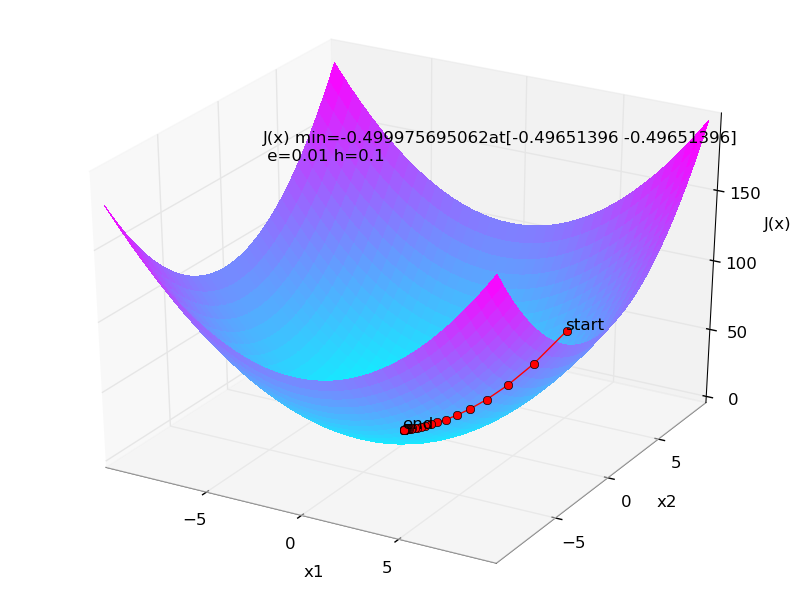
\includegraphics[width=8cm]{J1_1.png}&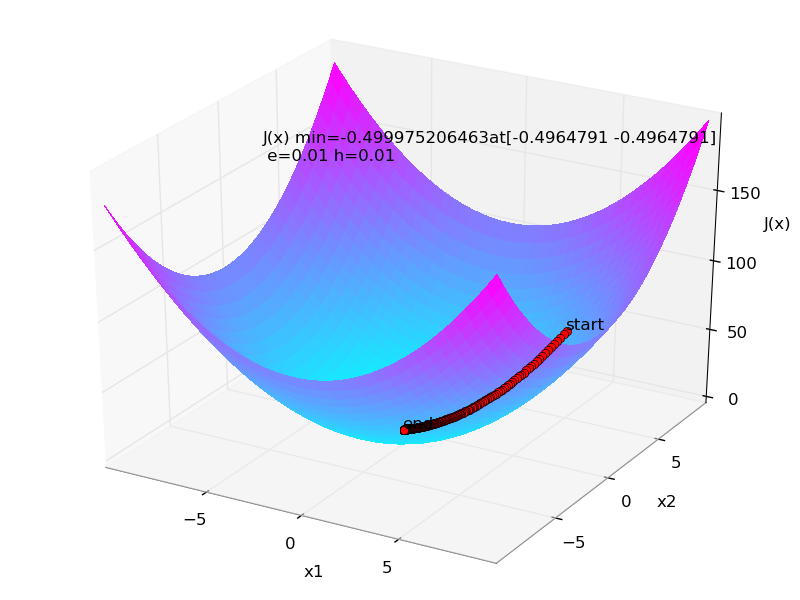
\includegraphics[width=8cm]{J1_2.png}\\
\hline
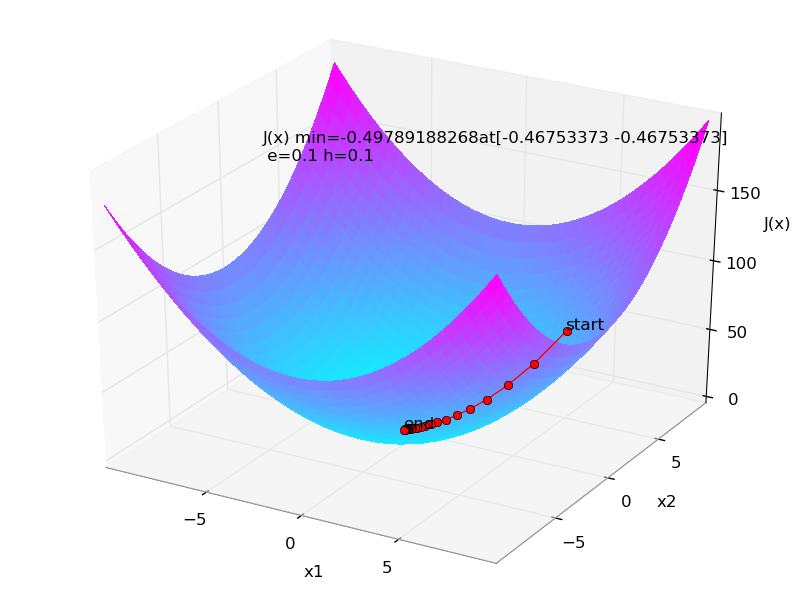
\includegraphics[width=8cm]{J1_3.png}&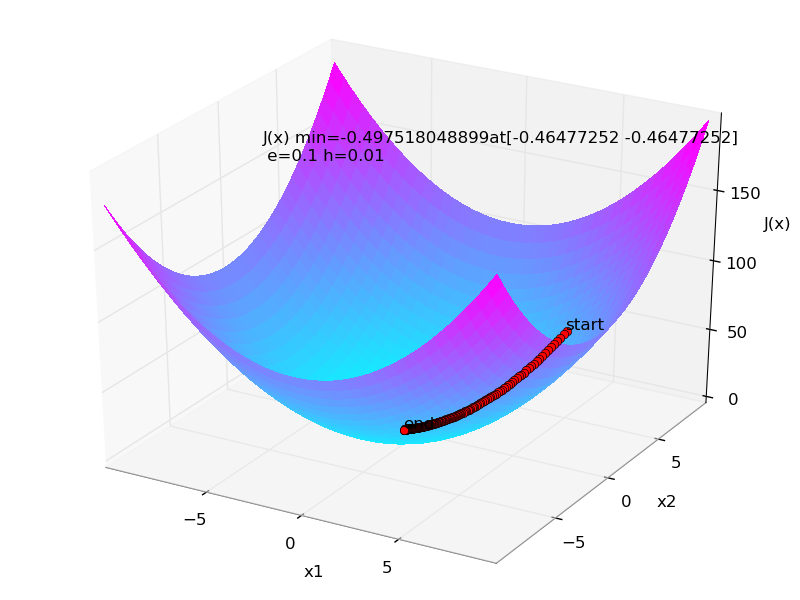
\includegraphics[width=8cm]{J1_4.png}\\
\hline
\end{tabular}
\caption{Visualization of $J_1(x)$ and Trajectory of Points Using Gradient Descent}
\label{J1}
\end{table}

\begin{table}[ht]
\centering
\begin{tabular}{|c|c|}
\hline
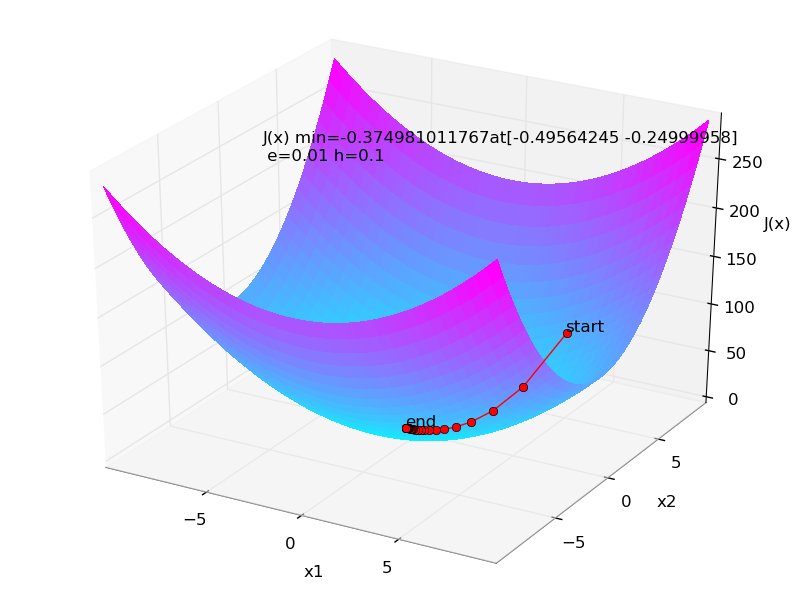
\includegraphics[width=8cm]{J2_1.png}&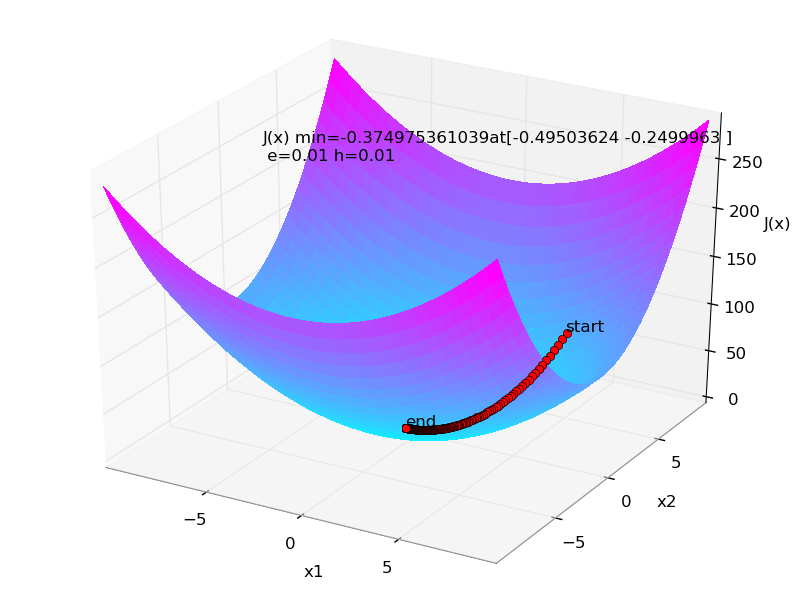
\includegraphics[width=8cm]{J2_2.png}\\
\hline
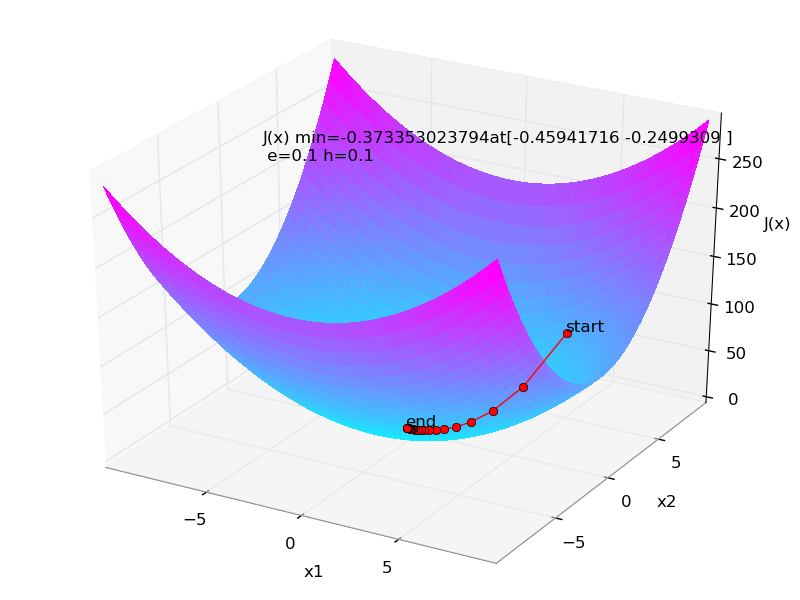
\includegraphics[width=8cm]{J2_3.png}&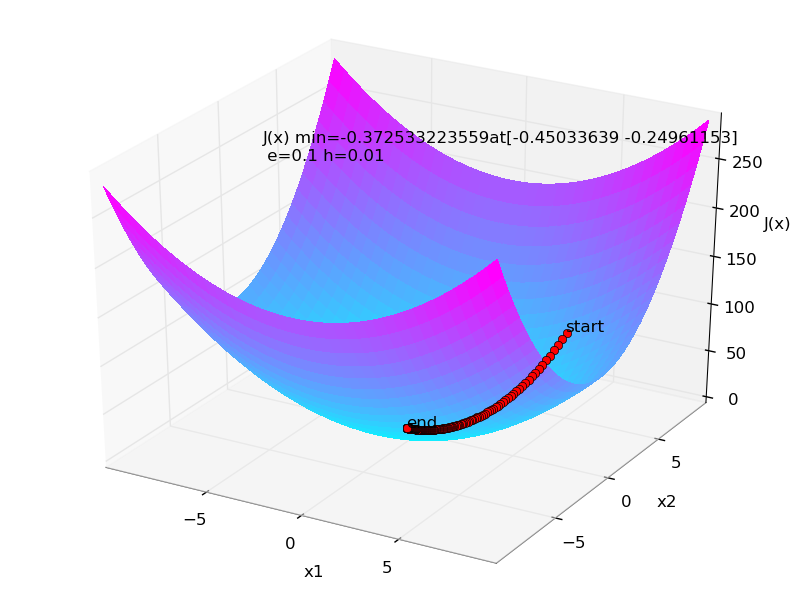
\includegraphics[width=8cm]{J2_4.png}\\
\hline
\end{tabular}
\caption{Visualization of $J_2(x)$ and Trajectory of Points Using Gradient Descent}
\label{J2}
\end{table}

\begin{table}[ht]
\centering
\begin{tabular}{|c|c|}
\hline
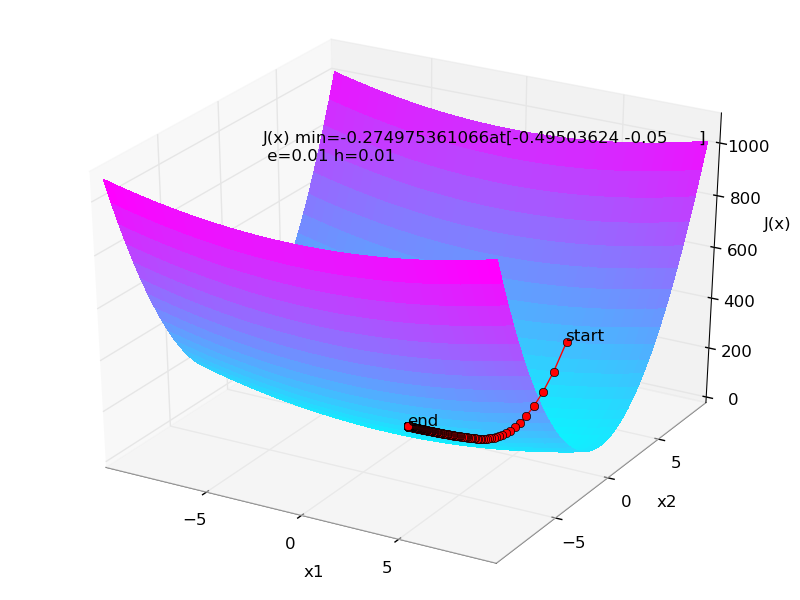
\includegraphics[width=8cm]{J3_1.png}&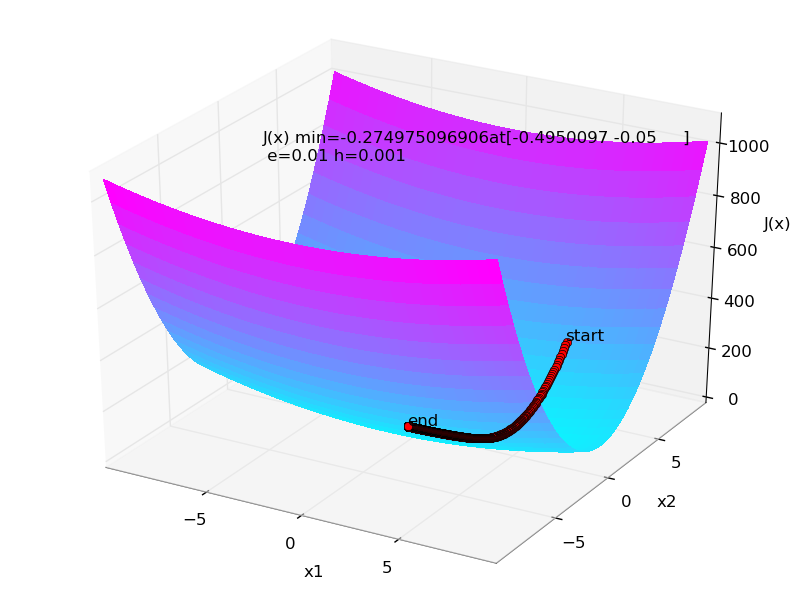
\includegraphics[width=8cm]{J3_2.png}\\
\hline
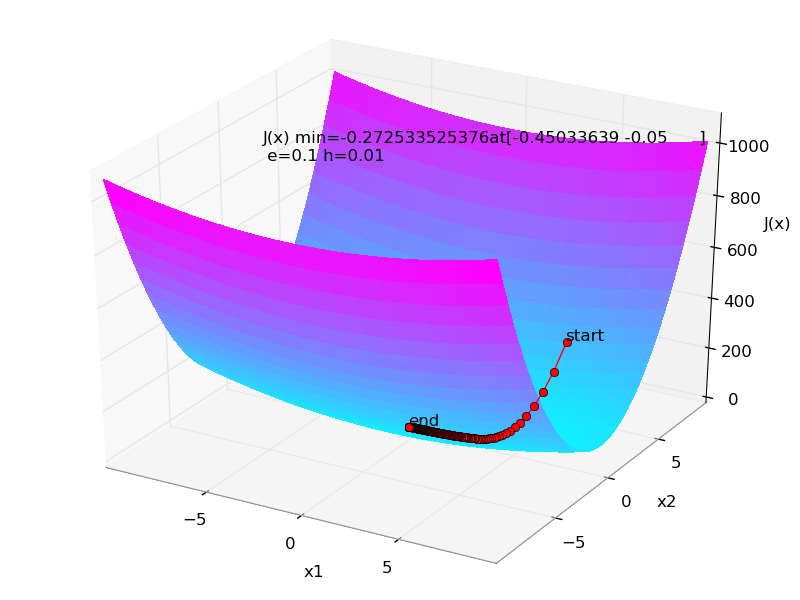
\includegraphics[width=8cm]{J3_3.png}&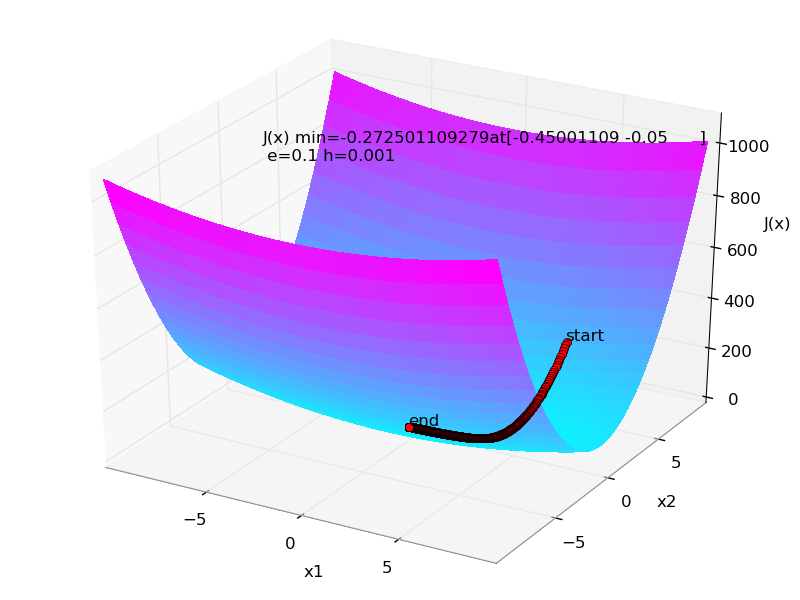
\includegraphics[width=8cm]{J3_4.png}\\
\hline
\end{tabular}
\caption{Visualization of $J_3(x)$ and Trajectory of Points Using Gradient Descent}
\label{J3}
\end{table}

\item Table \ref{JW} is showing the visualization of the objective function 
\[
J(w)=\frac{\lambda}{2} {\|w\|}^2 + \sum_i (w^Tx_i-y_i)^2
\]
with different values of $\lambda$'s. The first panel is showing $\lambda=0.001$.


\item See the red lines in Table \ref{JW} for different trajectories of points with $\lambda$'s $0.001$, $1.0$, $1000.0$, $100000.0$, $0.0001$, and $0.0$. Starting and ending points are marked in each panel. 

\item This function $J(w)$ is a combination of quadratic functions of $w$, we know that quadratic function is a convex function, thus $J(W)$ is also a convex function, which means if we can find a local minimum by gradient descent algorithm, that point is also the global minimum of that function. 

First of all, the choice of $\epsilon$ determines the accuracy of results, which is similar to the functions $J_1$, $J_2$, and $J_3$ above. 

Secondly, the choice of $\eta$ is determined by the $2,000$ data points we have. This big amount of data points makes the step size much larger than the cases in the previous functions $J_1$, $J_2$, or $J_3$. I tested on several different $\eta$'s, and found that $\eta=1e^{-5}$ is the optimal value in getting the minimum point in reasonable step numbers (I set the max iteration number to be $1000$).

Lastly, the choice of $\lambda$ makes a difference in the minimum of $J(w)$ only when $\lambda$ is huge. From 
\[
J(w)=\frac{\lambda}{2} {\|w\|}^2 + \sum_i (w^Tx_i-y_i)^2
\]
we know that the gradient of this function can be vectorized and put in Python code (see my code for reference):
\[
\nabla J(w) = \lambda w + 2 X^T (Xw-Y)
\]
Here $X$ is a $2000\times 2$ matrix of the $2,000$ data points; $Y$ is a $1000\times 1$ vector of the labels (either $+1$ or $-1$) of the $2,000$ dat points. When $\lambda$ is small, the first part $\lambda w$ is dominated by the second part $2 X^T (Xw-Y)$, as $X$ and $Y$ are huge matrices compared to the $2-d$ vector $w$; therefore in this case $\lambda$ almost has no impact on the gradient descent. However, when $\lambda$ gets larger, $w$ gets significantly important in determining $\nabla J(w_t)$. See summary results below of changes of $J(w)$ with different values of $\lambda$ (Please note that I used $h$ below instead of $\eta$ in my Python code). When $\lambda=100000.0$, the minimum moves from $[-0.11526332,-0.07674558]$ ($\lambda=0.001$) to $[5.94202596e+17,5.96931252e+17]$. 

\begin{verbatim}
Converged in  230 iterations
from [[ 1.]
 [ 1.]] to [[-0.11526332]
 [-0.07674558]]
J(w) min=1039.21825972at[[-0.11526332]
 [-0.07674558]] e=0.01 h=1e-05lamb=0.001

Converged in  230 iterations
from [[ 1.]
 [ 1.]] to [[-0.11525755]
 [-0.07674949]]
J(w) min=1039.22783777at[[-0.11525755]
 [-0.07674949]] e=0.01 h=1e-05lamb=1.0

Converged in  184 iterations
from [[ 1.]
 [ 1.]] to [[-0.11046043]
 [-0.07970587]]
J(w) min=1048.64285946at[[-0.11046043]
 [-0.07970587]] e=0.01 h=1e-05lamb=1000.0
from [[ 1.]
 [ 1.]] to [[  5.94202596e+17]
 [  5.96931252e+17]]
J(w) min=6.67348784196e+40at[[  5.94202596e+17]
 [  5.96931252e+17]] e=0.01 h=1e-05lamb=100000.0

Converged in  230 iterations
from [[ 1.]
 [ 1.]] to [[-0.11526333]
 [-0.07674558]]
J(w) min=1039.21825109at[[-0.11526333]
 [-0.07674558]] e=0.01 h=1e-05lamb=0.0001

Converged in  230 iterations
from [[ 1.]
 [ 1.]] to [[-0.11526333]
 [-0.07674558]]
J(w) min=1039.21825013at[[-0.11526333]
 [-0.07674558]] e=0.01 h=1e-05lamb=0.0
\end{verbatim}


\begin{table}[ht]
\centering
\begin{tabular}{|c|c|}
\hline
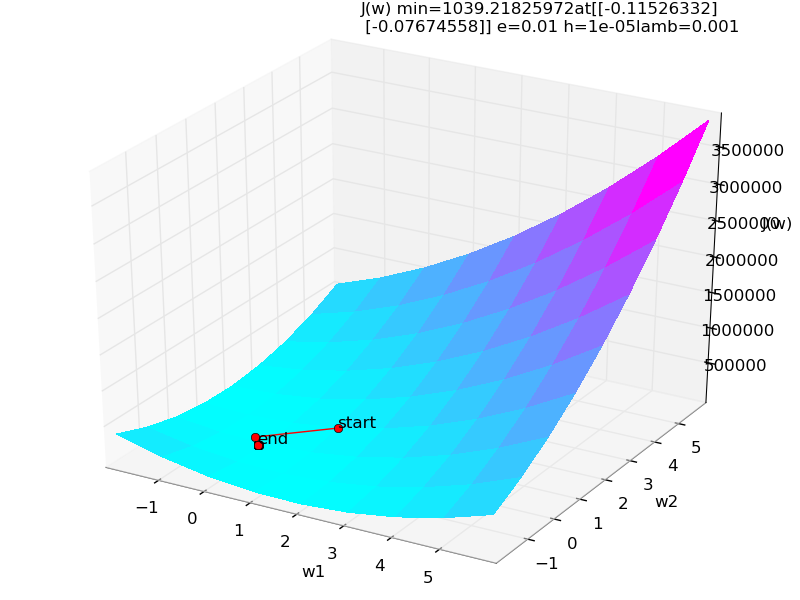
\includegraphics[width=8cm]{JW1.png}&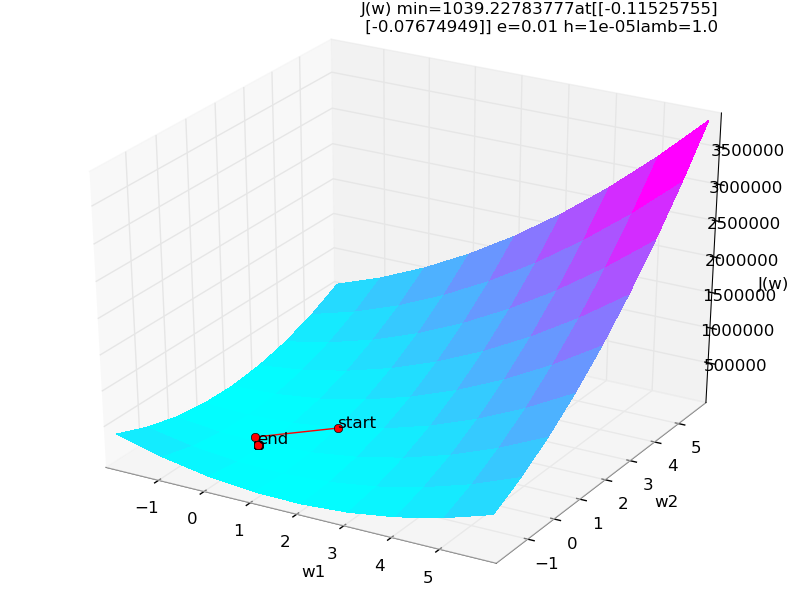
\includegraphics[width=8cm]{JW2.png}\\
\hline
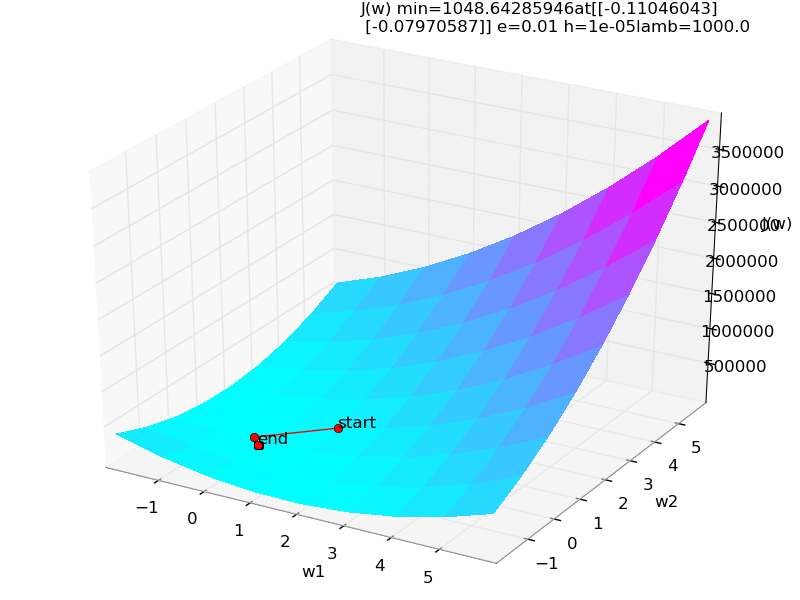
\includegraphics[width=8cm]{JW3.png}&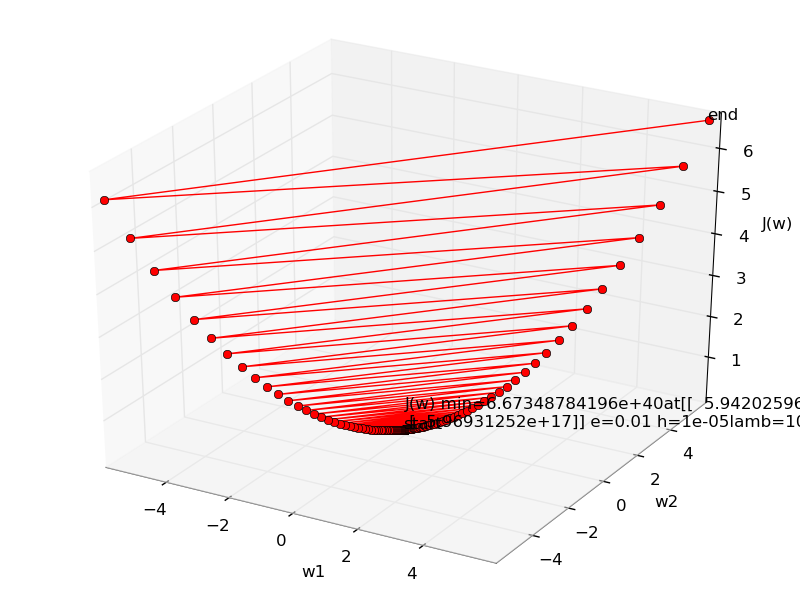
\includegraphics[width=8cm]{JW4.png}\\
\hline
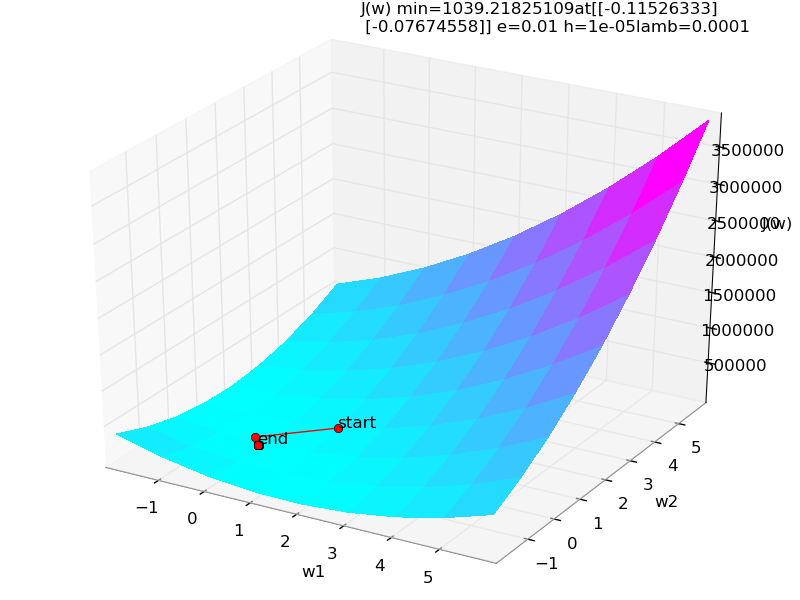
\includegraphics[width=8cm]{JW5.png}&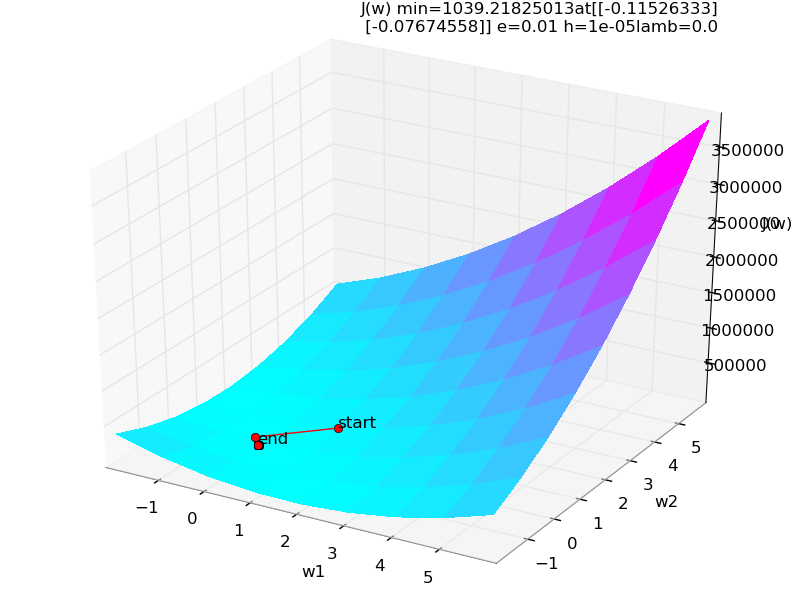
\includegraphics[width=8cm]{JW6.png}\\
\hline
\end{tabular}
\caption{Visualization of $J(w)$ and Trajectory of Points with $\lambda=0.001$, $1.0$, $1000.0$, $100000.0$, $0.0001$, and $0.0$}
\label{JW}
\end{table}


\end{itemize}

\end{document}